\documentclass{article}
\usepackage[utf8]{inputenc}

\usepackage{graphicx}
\graphicspath{ {./plots/} }
\usepackage{caption}
\usepackage{subcaption}


\title{Tennis Matches}

\begin{document}

\maketitle

% \tableofcontents

% TODO 
- DATA understanding
-   SCRIVERE
- DATA CLEANING
-   INDIVIDUARE PROBLEMI E PROPORRE POSSIBILI SOLUZIONI

\section{Introduction}

\subsection{Data understanding}
The \texttt{tennis\_matches} datset contains $186128$ total observations. Below the detailed analysis for each individual attribute.


\paragraph{toruney\_id}
The identifier of the tourney. On $186128$ observations, $55$ are missing. Every tourney is made up by multiple matches, hence the size of the tournament can be obtained, and on average there are . By analysing them, it's clear that the dataset is composed by different original sources. The ids can be categorized in three main groups:
\begin{itemize}
  \item length 8 and 9, such as \verb|2019-M020|. They are $44,6\%$ of the dataset and the first part gives information about the year of the tourney.
  \item length 23 and 24, such as \verb|2017-W-WITF-ARG-01A-2017|. They are $54\%$ of the dataset and the first part gives information about the year of the tourney, the country of the tourney, the woman category. Moreover for these there are additional informations available over the itftennis.com website. 
  \item length 30 to 40, such as \verb|2017-M-DC-2017-G2-AO-M-KUW-THA-01|. They are $1,2\%$ of the dataset and the first part gives information about the year of the tourney, the nationalities of the players.	
\end{itemize}


\paragraph{tourney\_name}
The name of the tourney. On $186103$ observations, $55$ are missing. Even here, different naming conventions provide different types of information.
\begin{itemize}
    \item \verb|Biella CH|. Gives information about the host city name.
    \item \verb|Arad $10K|. Gives information about the host city name, and the prize of the tournament. 
    \item \verb|W25 Rome|. In the case of the TF Women's World Tennis Tour, it gives information about the host city name and the category (i.e. W25). The latter states the number of events and the total prize for the category. The higher the number, the bigger the stakes.
    \item \verb|Fed Cup WG F: USA vs BLR| Gives information about the nationalities of the players.
\end{itemize}

\paragraph{surface}
The type of surface on which the players had the game. On $185940$ observations, $188$ are missing. The types are the following with their respective occurrences: Hard (95243), Clay (81044), Grass (6600), Carpet (3053).

\paragraph{draw\_size}
The number of players in the draw, that is often rounded up to the next power of $2$. The most common draw size for a tourney is $32$ followed by $2,4,64$. An overview can be seen in Fig.\ref{fig:draw_size_tourney}.
%TODO 5% of tourneys have a larger draw size than the player partecipating.


\begin{figure}[h]
\centering
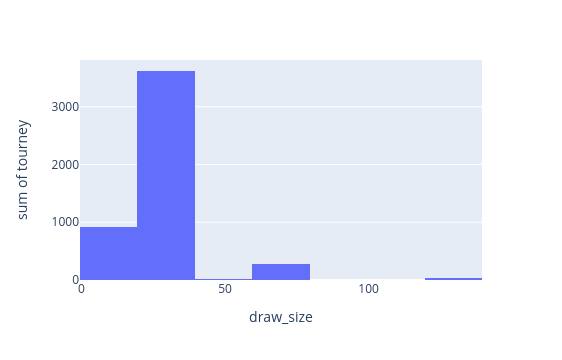
\includegraphics[width=.6\textwidth]{draw_size_tourney}
\captionof{figure}{Number of tourneys with a specific draw size}
\label{fig:draw_size_tourney}
\end{figure}


\paragraph{tourney\_level}
sdfhjsfjkhsafkalhsflkashflkahsdflkashjdkashjdkjsdfkjshdfk
sdfhjsfjkhsafkalhsflkashflkahsdflkashjdkashjdkjsdfkjshdfk
sdfhjsfjkhsafkalhsflkashflkahsdflkashjdkashjdkjsdfkjshdfk

- tourney_level -> da controllare con Tourney_name


\paragraph{tourney\_date}
The date of the tourney. On $186100$ observations of which $376$ are unique and $28$ are missing. The matches were disputed between the year $2016$ and $2021$, with most of them in the range $2016-2019$. For the months, instead, November and December tends to be the one with less matches. An overview of what has been said is shown in Fig.\ref{fig:matches_per_year} and Fig.\ref{fig:matches_per_year_and_month}. Moreover, the number of matches per day follows the distribution in Fig.\ref{fig:matches_per_day}.

\begin{figure}[h]
\centering
    \begin{minipage}{.5\textwidth}
        \centering
        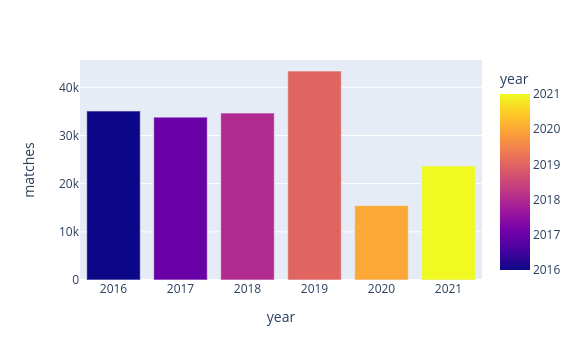
\includegraphics[width=\textwidth]{tourney_date_matches_per_year}
        \captionof{figure}{Matches per year}
        \label{fig:matches_per_year}
    \end{minipage}%
    \begin{minipage}{.5\textwidth}
        \centering
        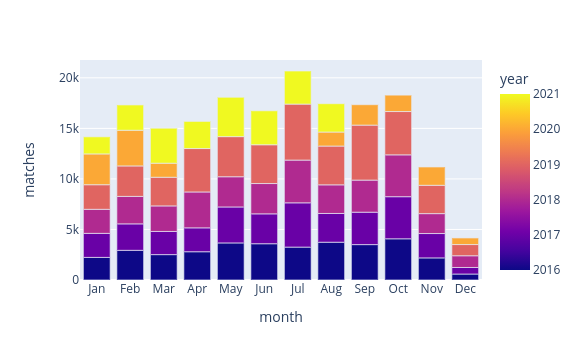
\includegraphics[width=\textwidth]{tourney_date_matches_per_year_and_month}
        \captionof{figure}{Matches per month/year}
        \label{fig:matches_per_year_and_month}
    \end{minipage}
    \begin{minipage}{.5\textwidth}
        \centering
        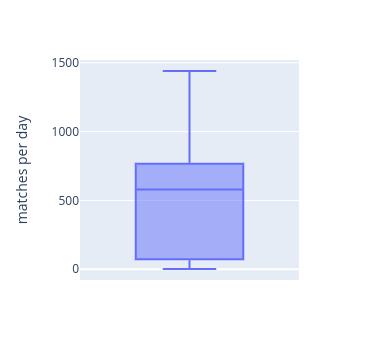
\includegraphics[width=.5\textwidth]{tourney_date_matches_per_day}
        \captionof{figure}{Matches per year}
        \label{fig:matches_per_day}
    \end{minipage}
\end{figure}

\newpage

Attributes:


++++++++++++++++++++++++++++++++++++++++++++++++++++++ 

\paragraph{match\_num}

- match_num -> valore che va parte da 0 o da 300 (se possibile distinguere l'occorrenza dei due casi)

\paragraph{winner\_id}

- winner_id -> capire se identifica giocatore in modo univoco o se lo identifica nel torneo

\paragraph{winner\_entry}

- Winner_entry -> analisi per capirne il significato semantico, tante missing

\paragraph{winner\_hand}

- winner_hand -> già ben definito (solo spiegare cos'è)

\paragraph{winner\_name}

- winner_name -> analisi più approfondita per capire se ci sono problemi

\paragraph{winner\_ht}

- winner_ht -> outlier e tante missing

\paragraph{winner\_ioc}

- Winner_ioc -> tutto ben definito apparte missing

\paragraph{winner\_age}

- Winner_age -> outlier e distribuzion

\paragraph{loser\_id}

- loser_id -> uguale ad il winner_id

\paragraph{loser\_entry}

- loser_entry ->  uguale ad il Winner_entry

\paragraph{loser\_name}

- loser_name -> uguale al winner_name

\paragraph{loser\_hands}

- loser_hands -> uguale al winner_hands

\paragraph{loser\_ht}

- loser_ht -> uguale a winner_ht

\paragraph{loser\_ioc}

- loser_ioc -> uguale a Winner_ioc

\paragraph{loser\_age}

- loser_age -> uguale a Winner_age

\paragraph{round}

An acronym which identifies the stage of the match inside the competition.


++++++++++++++++++++++++++++++++++++++++++++++++++++++

- score -> spiegato il significato semantico e spiegare il tipo di pattern che si trovano

- best_of -> formattato bene

- minutes -> tutti interi, analisi distribuzione

- w_ace -> tutti numerici

- W_df -> tutti numerici

- W_svpt

- W_1stln

- W_1stWon

- W_2stwon

- W_SvGms

- W_bdSaved

- W_bdFaced

- Winner_rank

- Winner_rank_points





\end{document}

